\documentclass[a4paper,14pt]{extarticle} 
\usepackage[a4paper,top=1.5cm, bottom=1.5cm, left=2cm, right=1cm]{geometry}
%\usepackage[T2A]{fontenc}
%\usepackage[english, russian]{babel}
\usepackage{graphicx}
\DeclareGraphicsExtensions{.pdf,.png,.jpg}

\usepackage{fontspec}
\setmainfont{Times New Roman}
\setsansfont{FreeSans}
\setmonofont{FreeMono}
\renewcommand{\baselinestretch}{1.5}
\usepackage{polyglossia}
\setdefaultlanguage{russian}
\setotherlanguages{english,russian}
\usepackage{setspace}
\usepackage[many]{tcolorbox}
\usepackage{listings}
\usepackage{xcolor}
\usepackage{pdfpages}

\definecolor{codegreen}{rgb}{0,0.6,0}
\definecolor{codegray}{rgb}{0.5,0.5,0.5}
\definecolor{codepurple}{rgb}{0.58,0,0.82}
\definecolor{backcolour}{rgb}{0.95,0.95,0.92}

\lstdefinestyle{mystyle}{
    backgroundcolor=\color{backcolour},   
    keywordstyle=\color{magenta},
    numberstyle=\tiny\color{codegray},
    stringstyle=\color{codepurple},
    basicstyle=\ttfamily\footnotesize,
    breakatwhitespace=false,         
    breaklines=true,                 
    captionpos=b,                    
    keepspaces=true,                 
    numbers=left,                    
    numbersep=5pt,                  
    showspaces=false,                
    showstringspaces=false,
    showtabs=false,                  
    tabsize=2
}

\lstset{style=mystyle}

\begin{document}
    \begin{center}
        \thispagestyle{empty}
        \begin{singlespace}
        ФЕДЕРАЛЬНОЕ АГЕНТСТВО СВЯЗИ

        ФЕДЕРАЛЬНОЕ ГОСУДАРСТВЕННОЕ БЮДЖЕТНОЕ ОБРАЗОВАТЕЛЬНОЕ

        УЧРЕЖДЕНИЕ ВЫСШЕГО ОБРАЗОВАНИЯ

        «САНКТ-ПЕТЕРБУРГСКИЙ ГОСУДАРСТВЕННЫЙ УНИВЕРСИТЕТ ТЕЛЕКОММУНИКАЦИЙ ИМ. ПРОФ. М.А. БОНЧ-БРУЕВИЧА»

        (СПбГУТ)
        \end{singlespace}
        \vspace{-1ex}
        \rule{\textwidth}{0.4pt}
        \vspace{-5ex}

        Факультет \underline{Инфокоммуникационных сетей и систем}

        Кафедра \underline{Защищенных систем связи}
        \vspace{10ex}

        \textbf{Лабораторная работа №1}\\
        


    \end{center}
    \vspace{4ex}
    \begin{flushright}
    \parbox{10 cm}{
    \begin{flushleft}
        Выполнили студенты группы ИКТЗ-83:

        \underline{Громов А.А., Миколаени М.С., Мазеин Д.С.} \hfill \rule[-0.85ex]{0.1\textwidth}{0.6pt}

        \footnotesize \textit{ (Ф.И.О., № группы) \hfill (подпись)} \normalsize

        Проверил:

        \underline{Казанцев А.А.} \hfill \rule[-0.85ex]{0.1\textwidth}{0.6pt}

        (\footnotesize \textit{уч. степень, уч. звание, Ф.И.О.) \hfill (подпись)} \normalsize

    \end{flushleft}
    }
    \end{flushright}
    \begin{center}
        \vfill
        Санкт-Петербург

        2021

    \end{center}
    \newpage

    \textbf{Цель лабораторной работы:}

    Перенести в autocad, добавить систему охраны:
    \vspace{-6ex}
    \begin{singlespace}
        \begin{itemize}
            \item расположить охранные датчики,
            \item расположить камеры, 
            \item расположить СКУД.
        \end{itemize} 
    \end{singlespace}

    \textbf{Схема помещения:}
    \begin{center}
        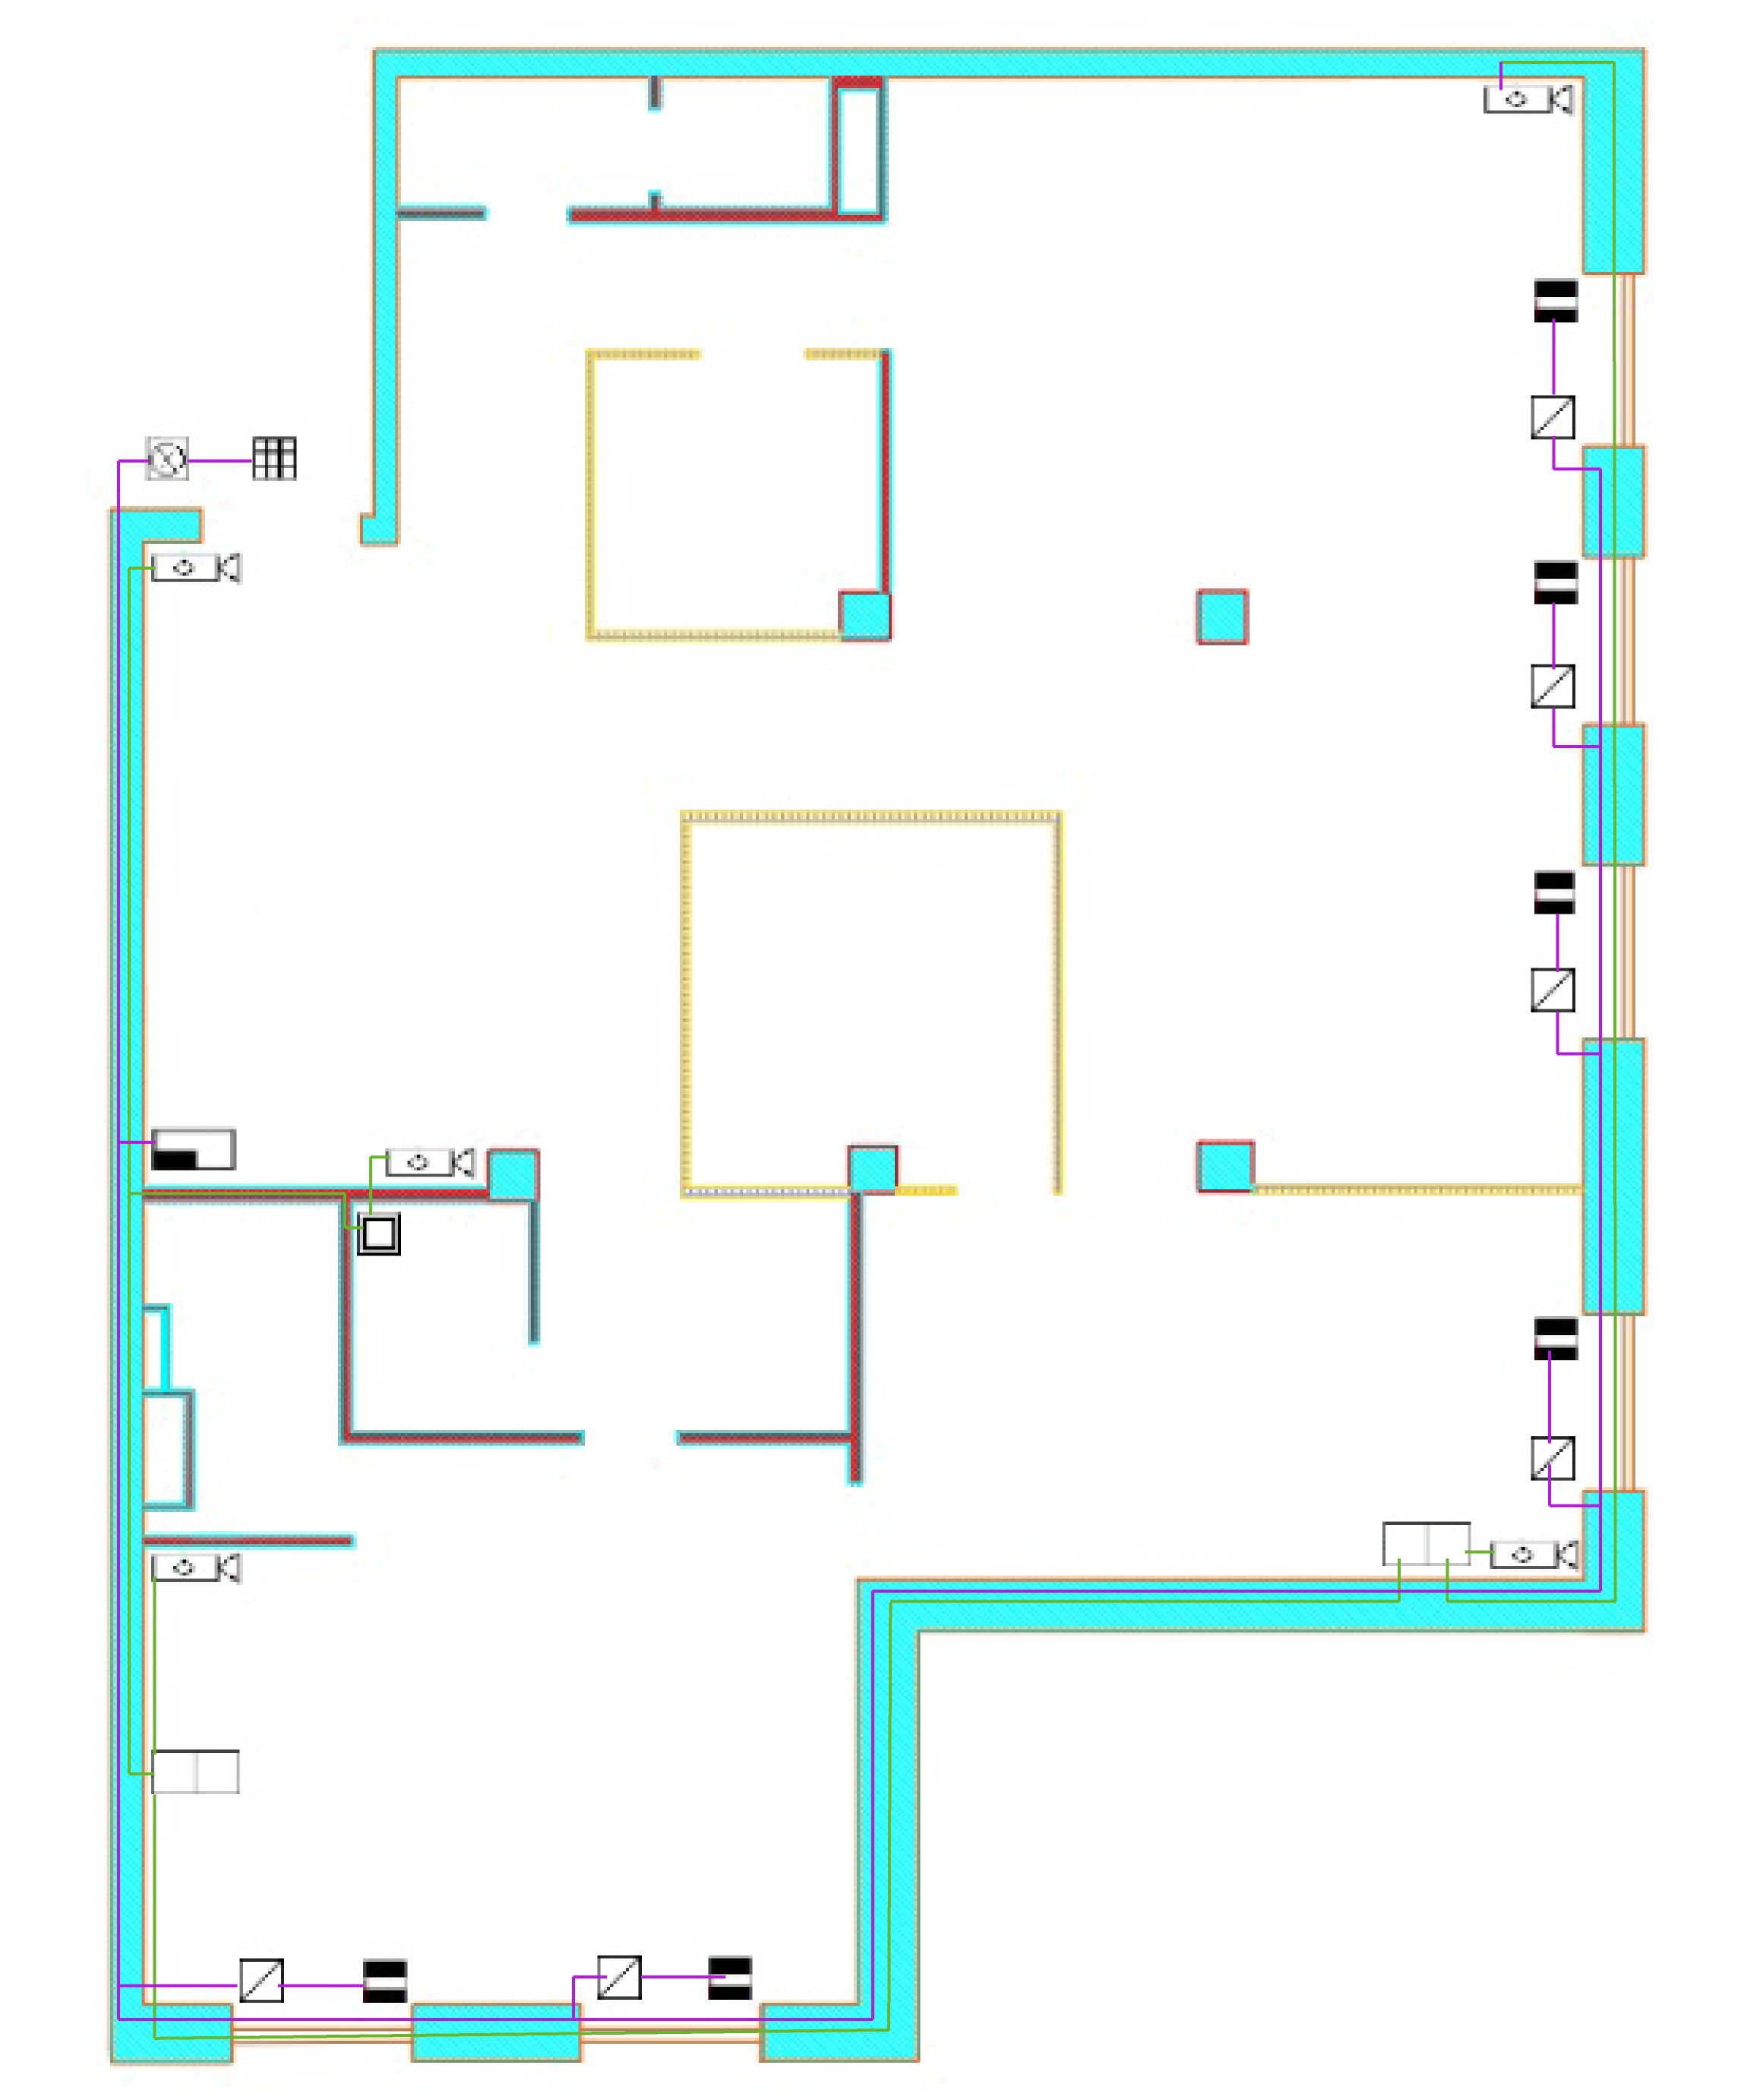
\includegraphics[scale=0.6, angle=90]{pics/scheme.png}
    \end{center}

    \newpage
    \textbf{\large{Охранная сигнализация}}

    \begin{center}
        \textbf{Схема}
    \end{center}
    \vspace{-6ex}
    \begin{center}
        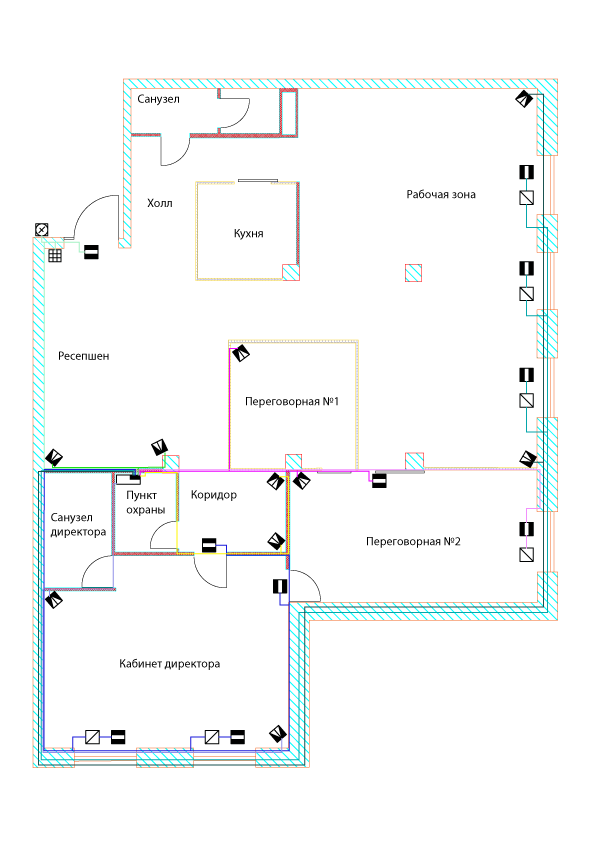
\includegraphics[scale=0.65, angle=90]{pics/Sensors.png}
    \end{center}
    \textbf{Условные обозначения}
    \begin{center}
        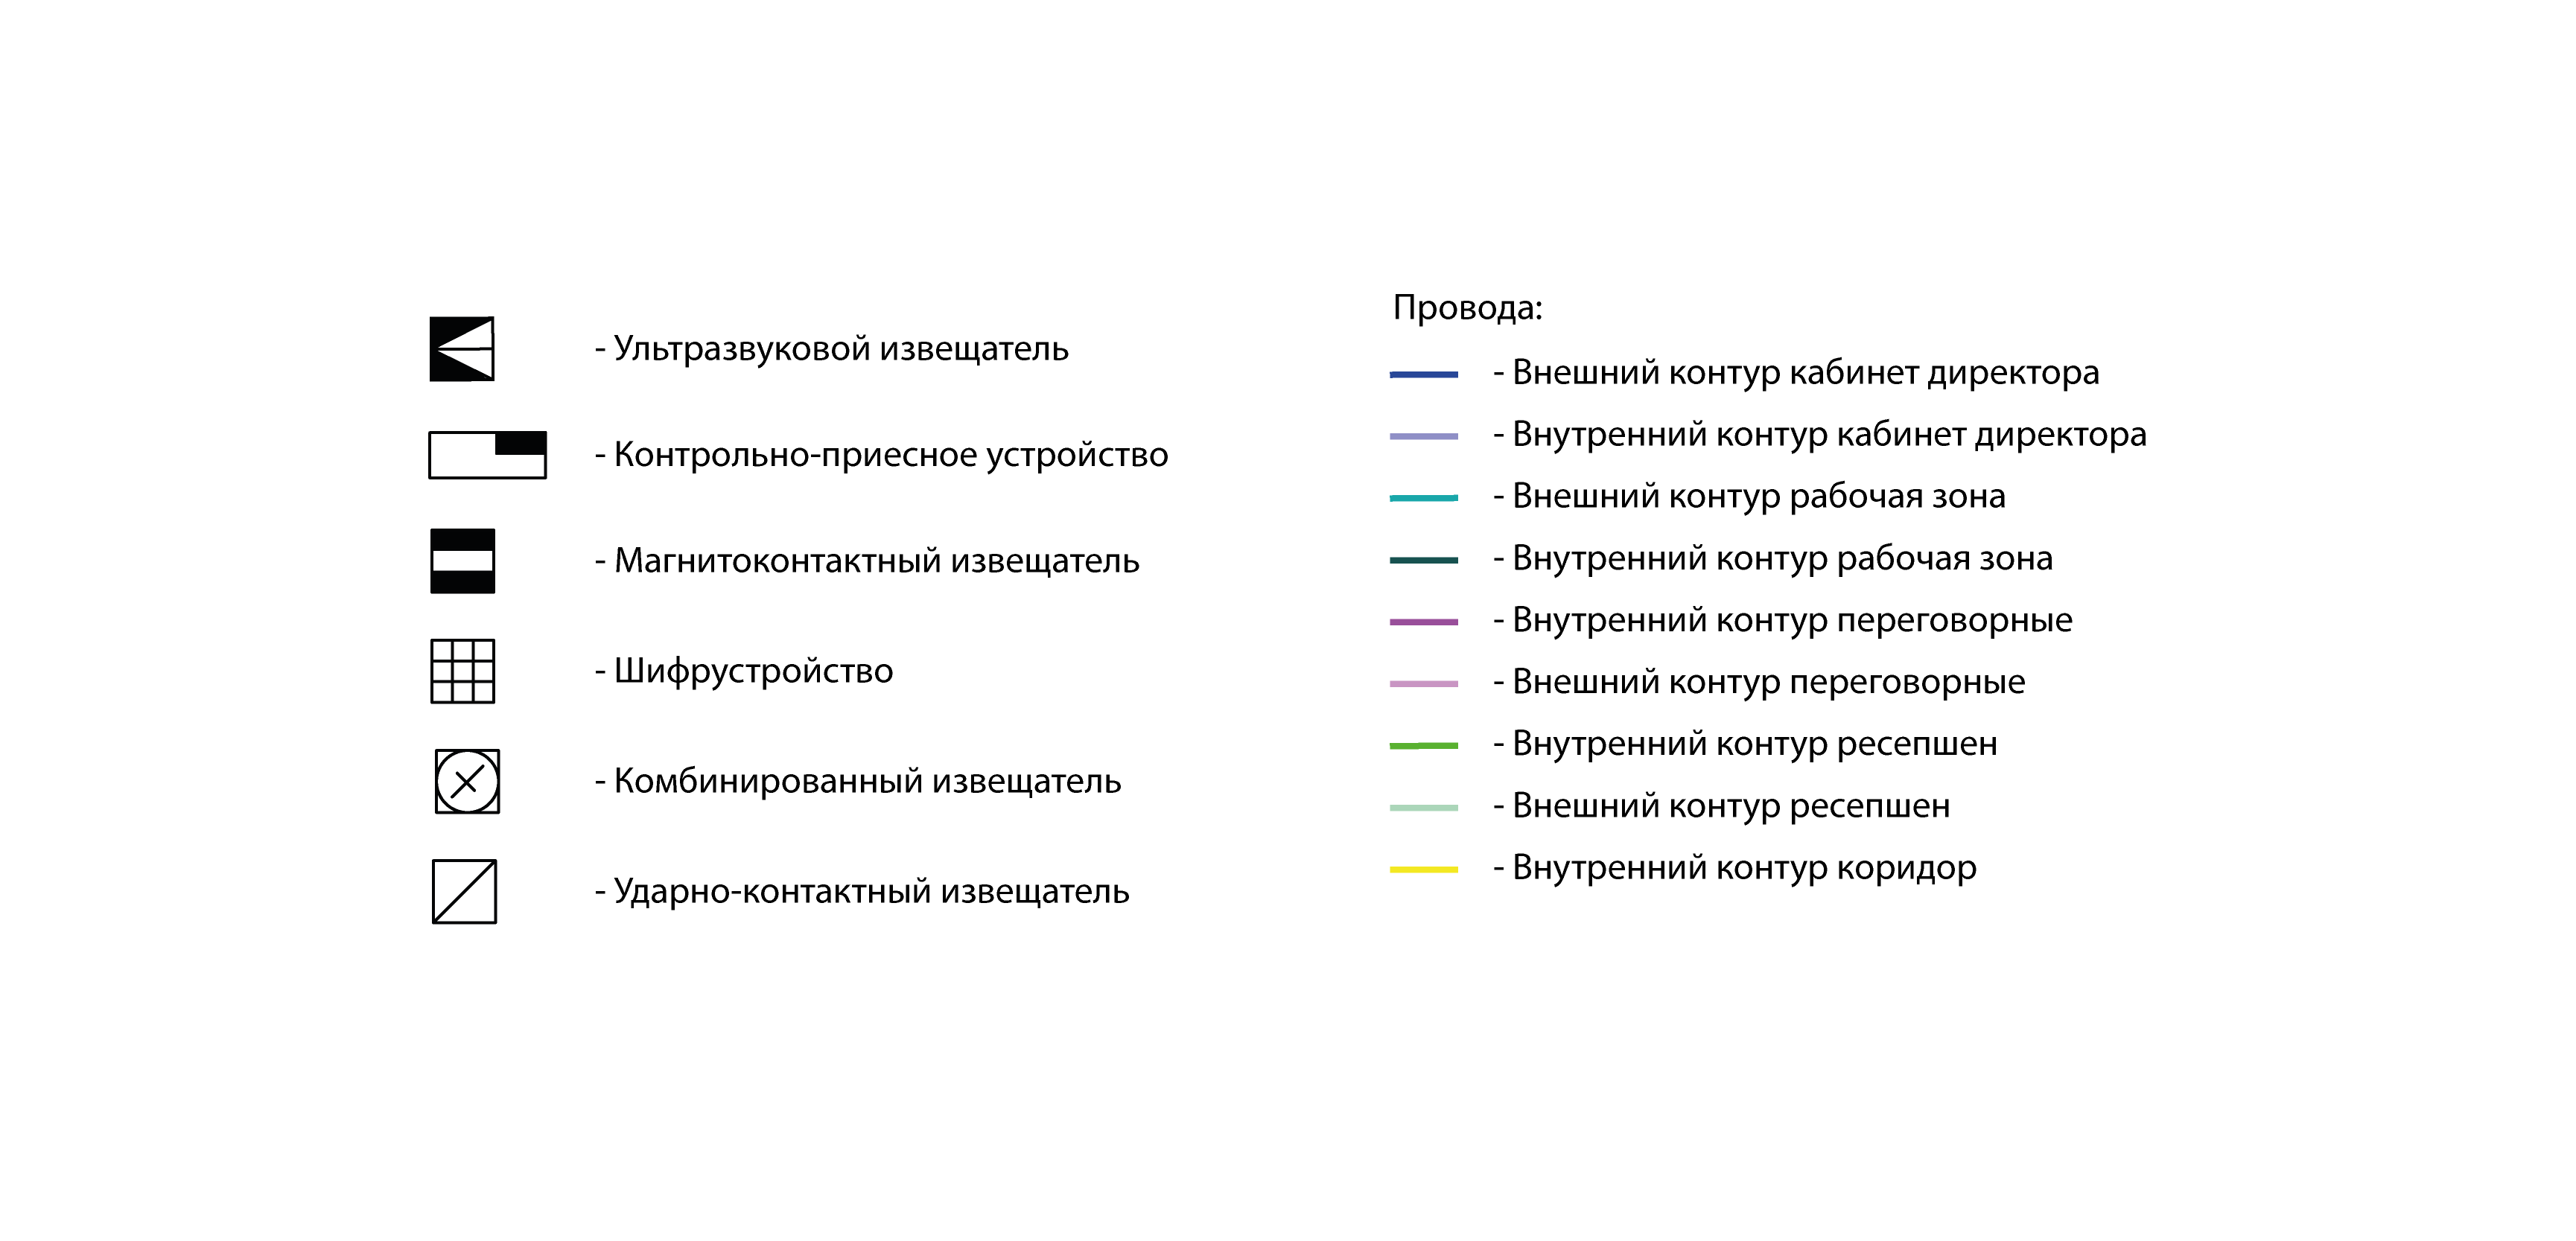
\includegraphics[scale=0.65]{pics/Sensors(mark).png}
    \end{center}
    \textbf{Пояснительная записка}
    \begin{spacing}{1.25}
        Офисное помещение разделено на 5 зоны:
        \vspace{-1ex}
        \begin{spacing}{0.5}
            \begin{itemize}
                \item рабочая зона;
                \item ресепшн;
                \item переговорные; 
                \item коридор;
                \item кабинет директора;
            \end{itemize}
        \end{spacing}
        Разделение на зоны обусловлено тем, что датчики подключены последовательно. В связи с этим, при срабатывании одного из датчиков в цепи, на контрольно-приемном устройстве будет сложно определить место проникновения злоумышленника. С этим также связано разделение на контуры. Таким образом мы увеличиваем точность определения прорыва периметра охраняемой территории/помещения.

        Рабочая зона защищена ударно-контактными и магнитоконтактными извещателями по внешнему контуру. Это обеспечивает защиту от проникновения в помещение через окна.

        Внутренний контур оснащен ультразвуковыми излучателями, обнаруживающими движение в охраняемой зоне. Данный тип извещателей выбран потому, что он использует ультразвуковые волны для отслеживания изменения объема, в отличии от инфракрасных, тепловых или звуковых датчиков. У выбранных датчиков также наблюдается наименьший риск ложного срабатывания. 

        В остальных зонах (кроме коридора) соблюдается тот же принцип установки датчиков. 

        Ресепшн дополнительно оборудован комбинированным извещателем, установленным снаружи за входной дверью, а также шифроустройством для того, чтобы первый пришедший сотрудник мог снять объект с охраны. 

        В коридоре установлены ультразвуковые излучатели, которые следят за движением в самых критичных зонах - пункт охраны и кабинет директора.
    \end{spacing}
    
    \newpage
    \textbf{\large{Система видеонаблюдения}}

    \begin{center}
        \textbf{Схема}
    \end{center}
    \vspace{-6ex}
    \begin{center}
        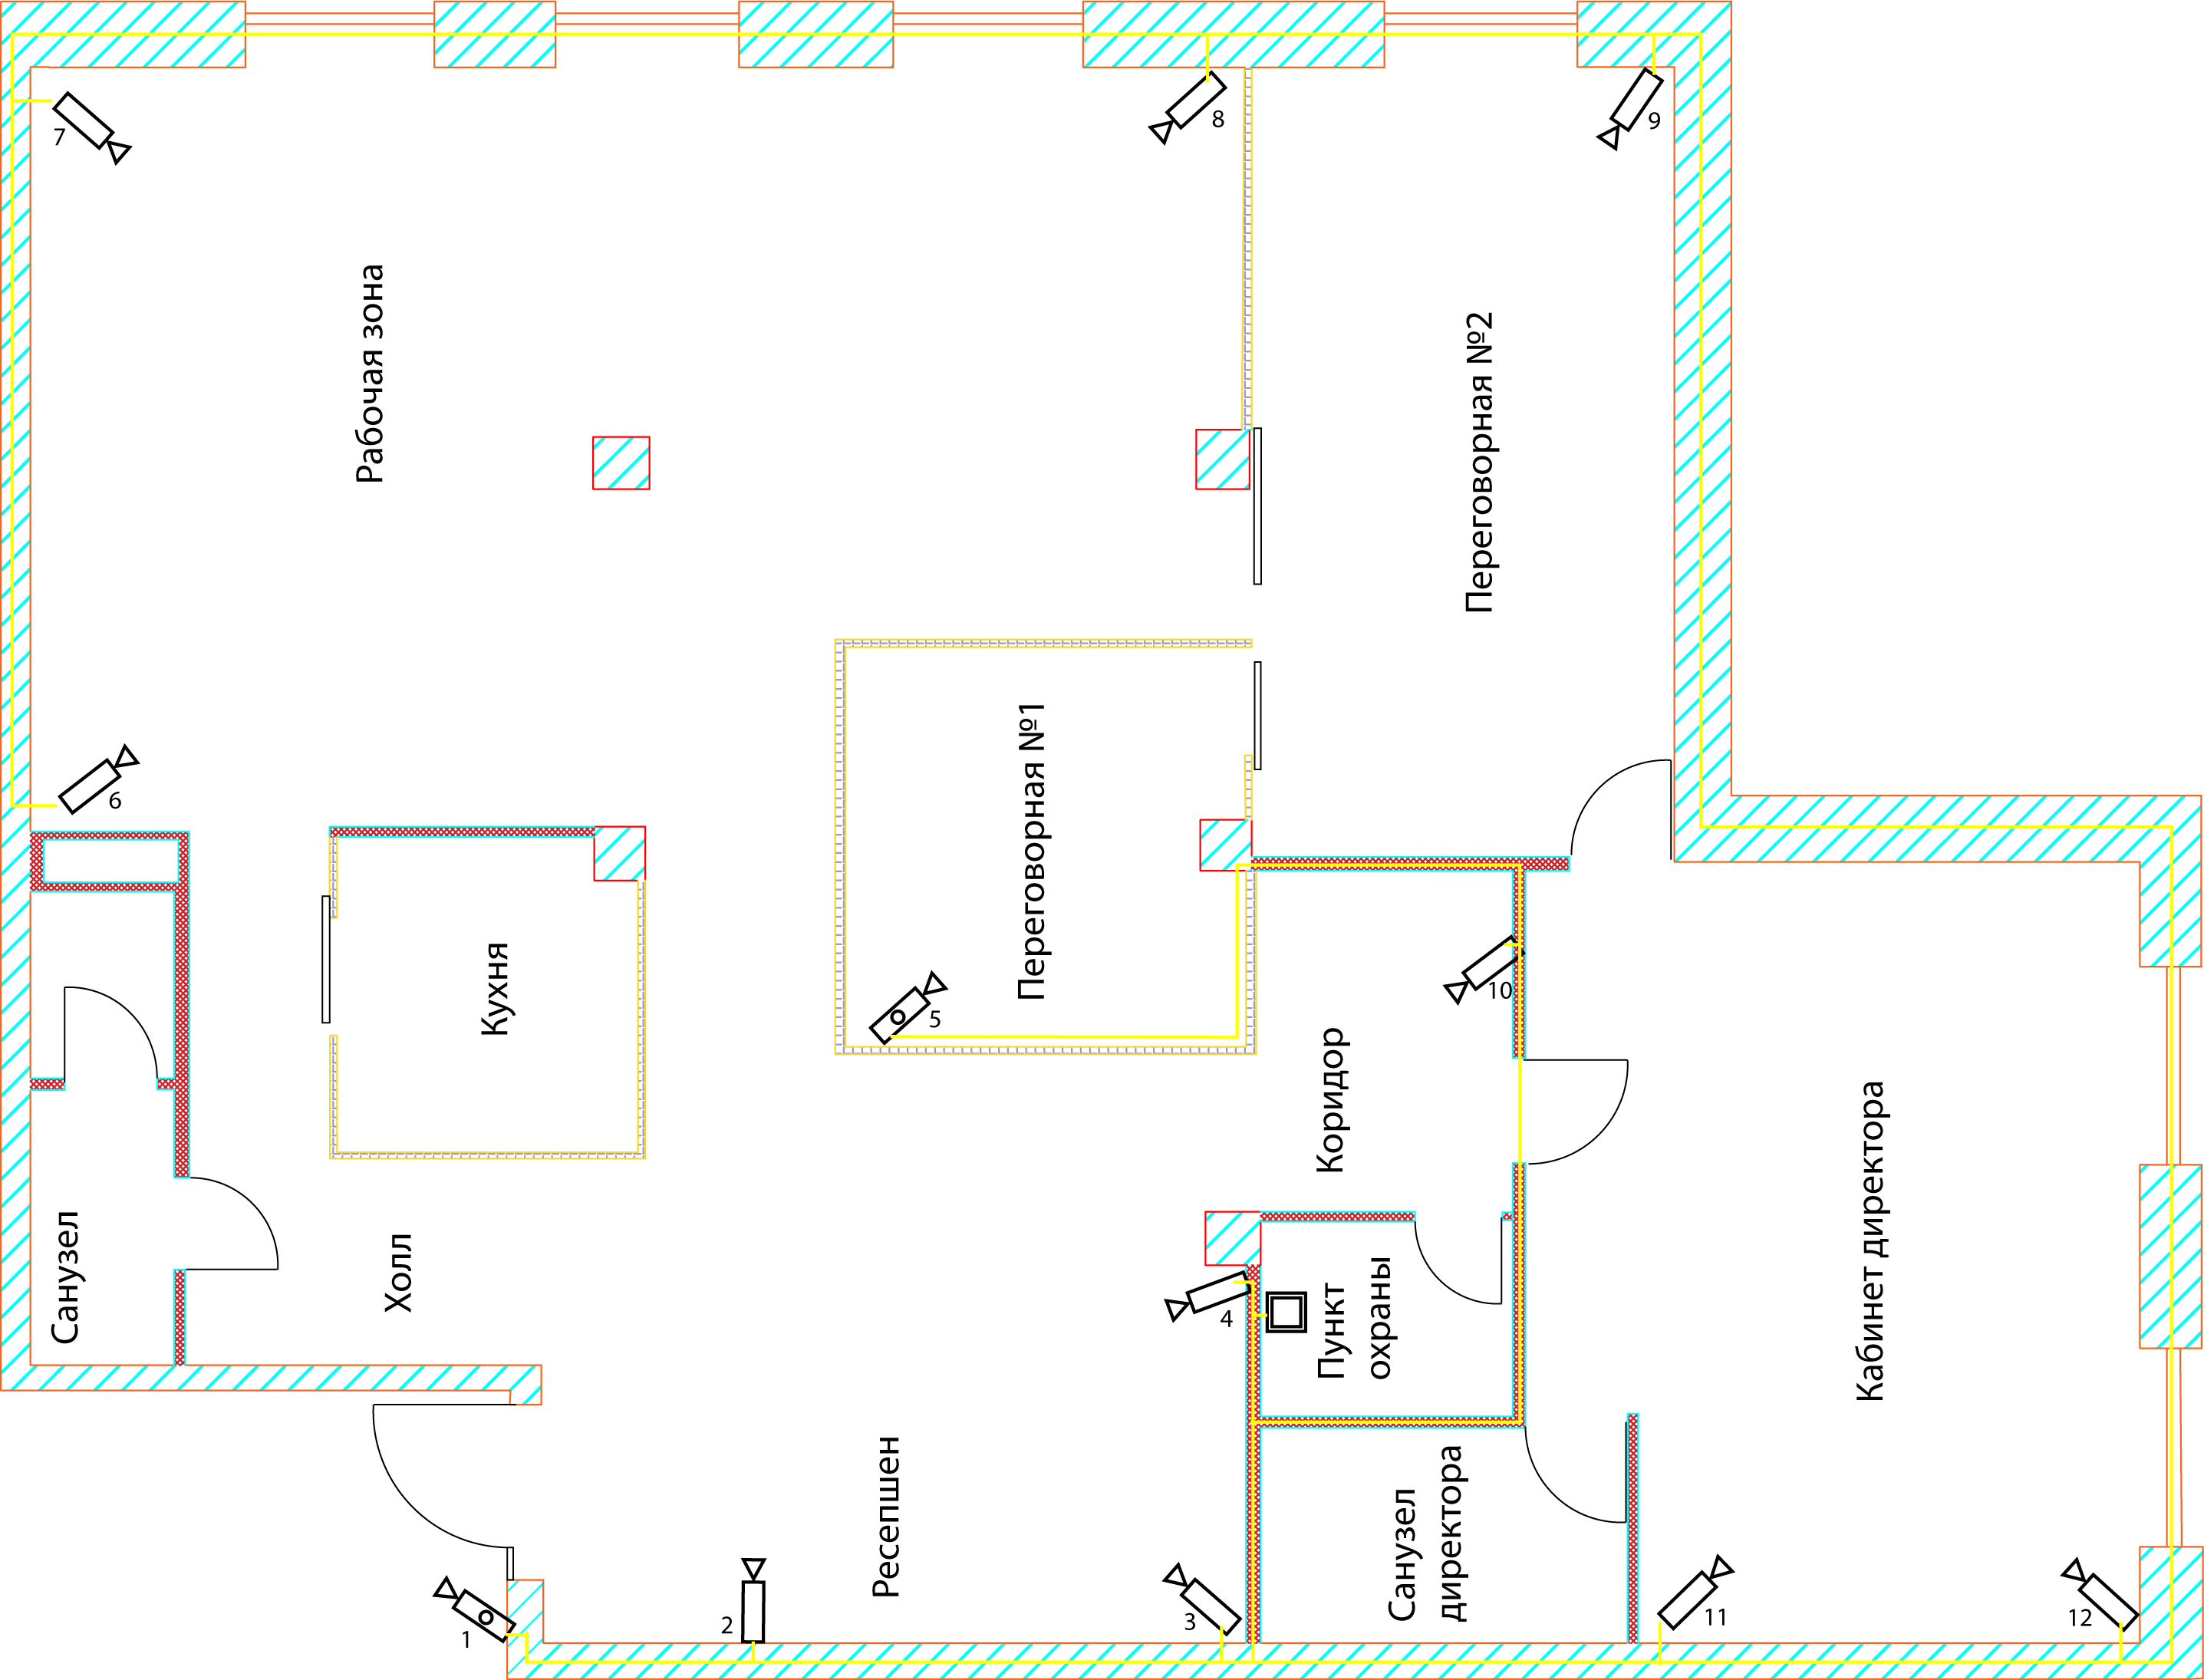
\includegraphics[scale=0.65]{pics/Cams.png}
    \end{center}
    \textbf{Условные обозначения}
    \begin{center}
        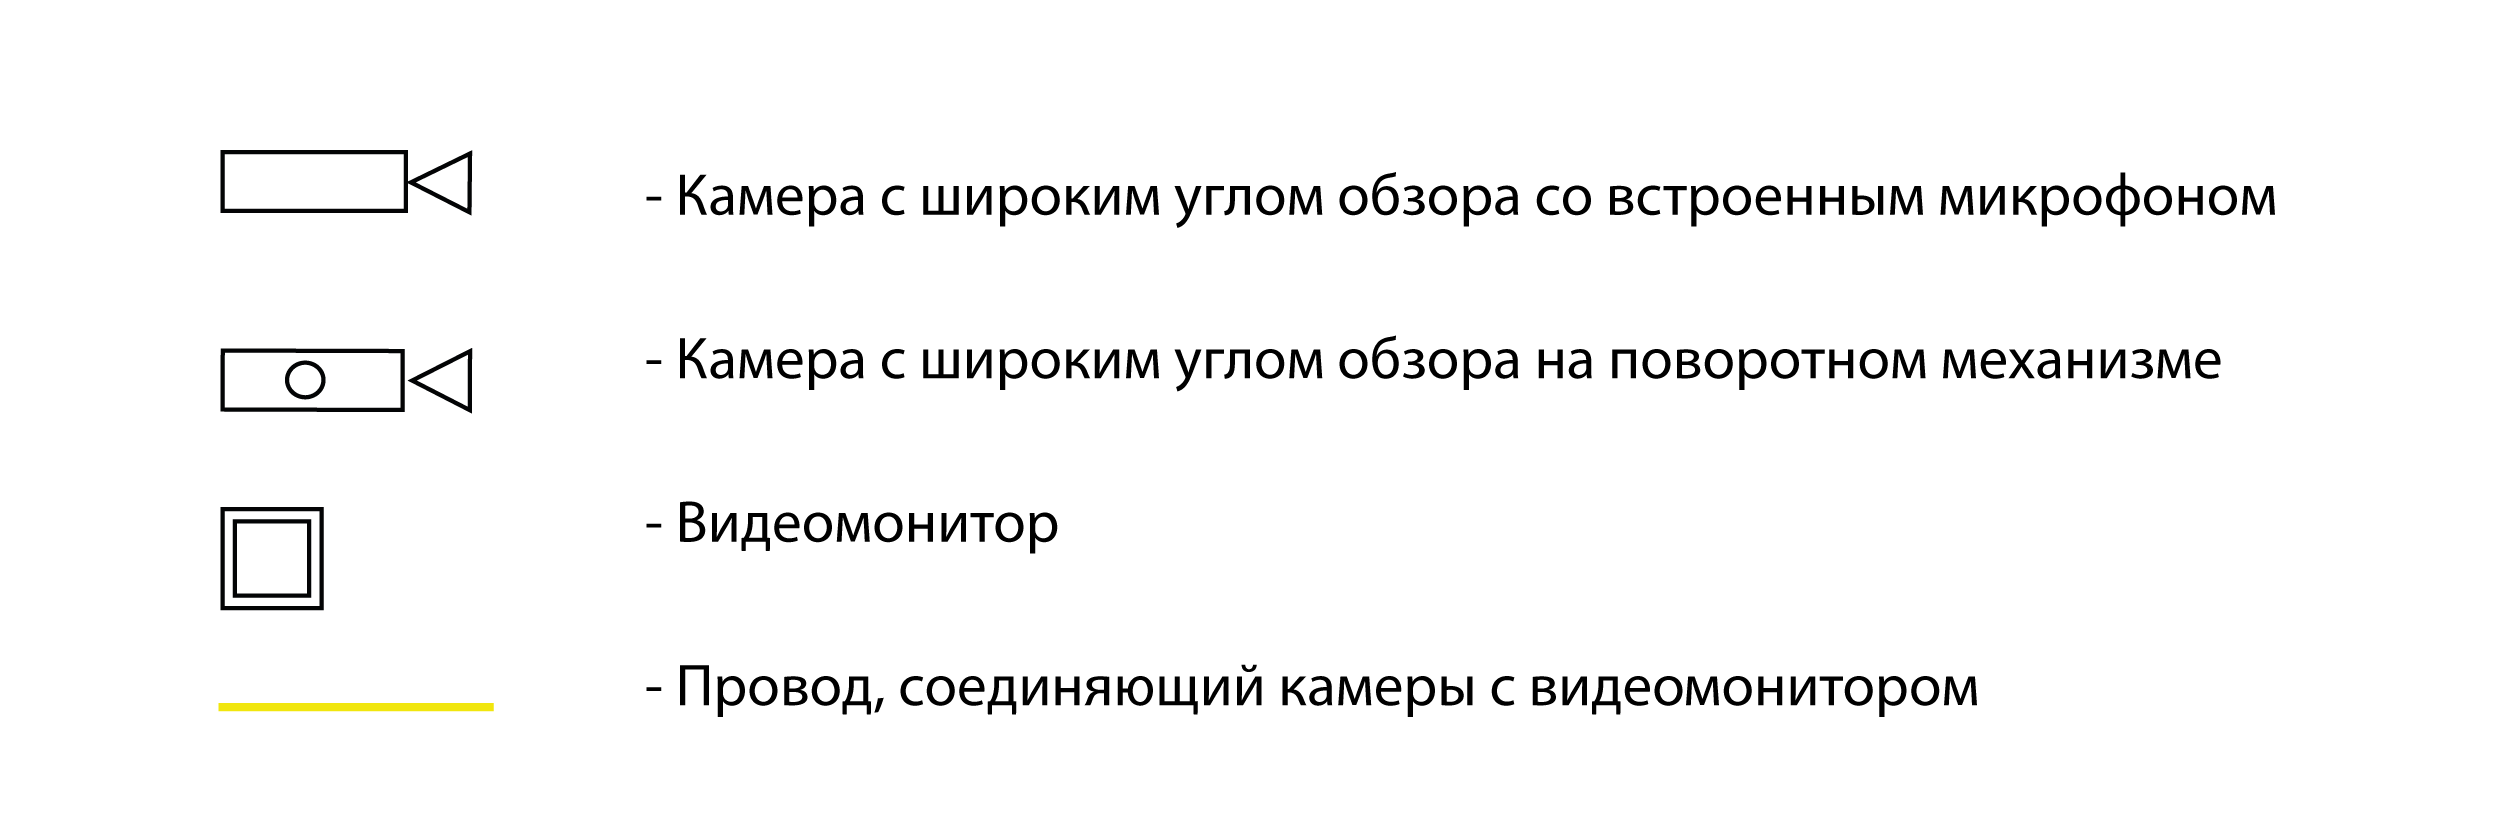
\includegraphics[scale=0.65]{pics/Cams(mark).png}
    \end{center}
    \textbf{Пояснительная записка}
    \begin{spacing}{1.25}
        Поворотная камера на входе (1) позволяет отслеживать подходящих к входной двери людей.

        Камеры, установленные на ресепшене просматривают коридор между кухней и переговорной №1 (2), холл (3), а также контролируют входную дверь (4).

        Камеры, расположенные в рабочей зоне (6, 7, 8) отслеживают перемещения сотрудников на рабочих местах. 

        Камеры, установленные в переговорных (5, 9) позволяют наблюдать за людьми, которые находятся в данных комнатах.

        Камера в коридоре (10)  контролирует проход к пункту охраны и кабинету директора.

        Камеры, в кабинете директора позволяют отслеживать действия лиц, находящихся в кабинете (12), а также происходящее за окнами офиса (11). 
    \end{spacing}

    \newpage
    \textbf{\large{Система контроля и управления доступом}}

    \begin{center}
        \textbf{Схема}
    \end{center}
    \vspace{-6ex}
    \begin{center}
        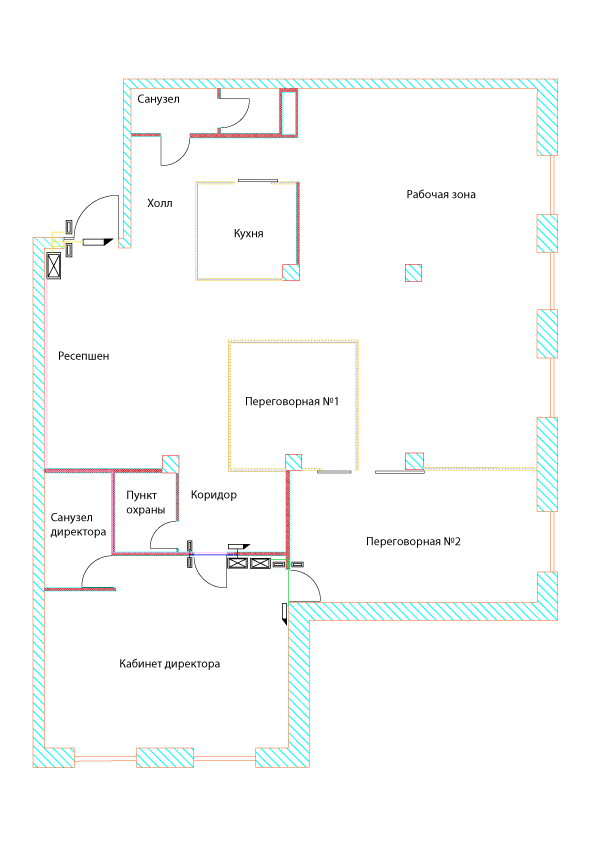
\includegraphics[scale=0.65, angle=90]{pics/SCUD.png}
    \end{center}
    \textbf{Условные обозначения}
    \begin{center}
        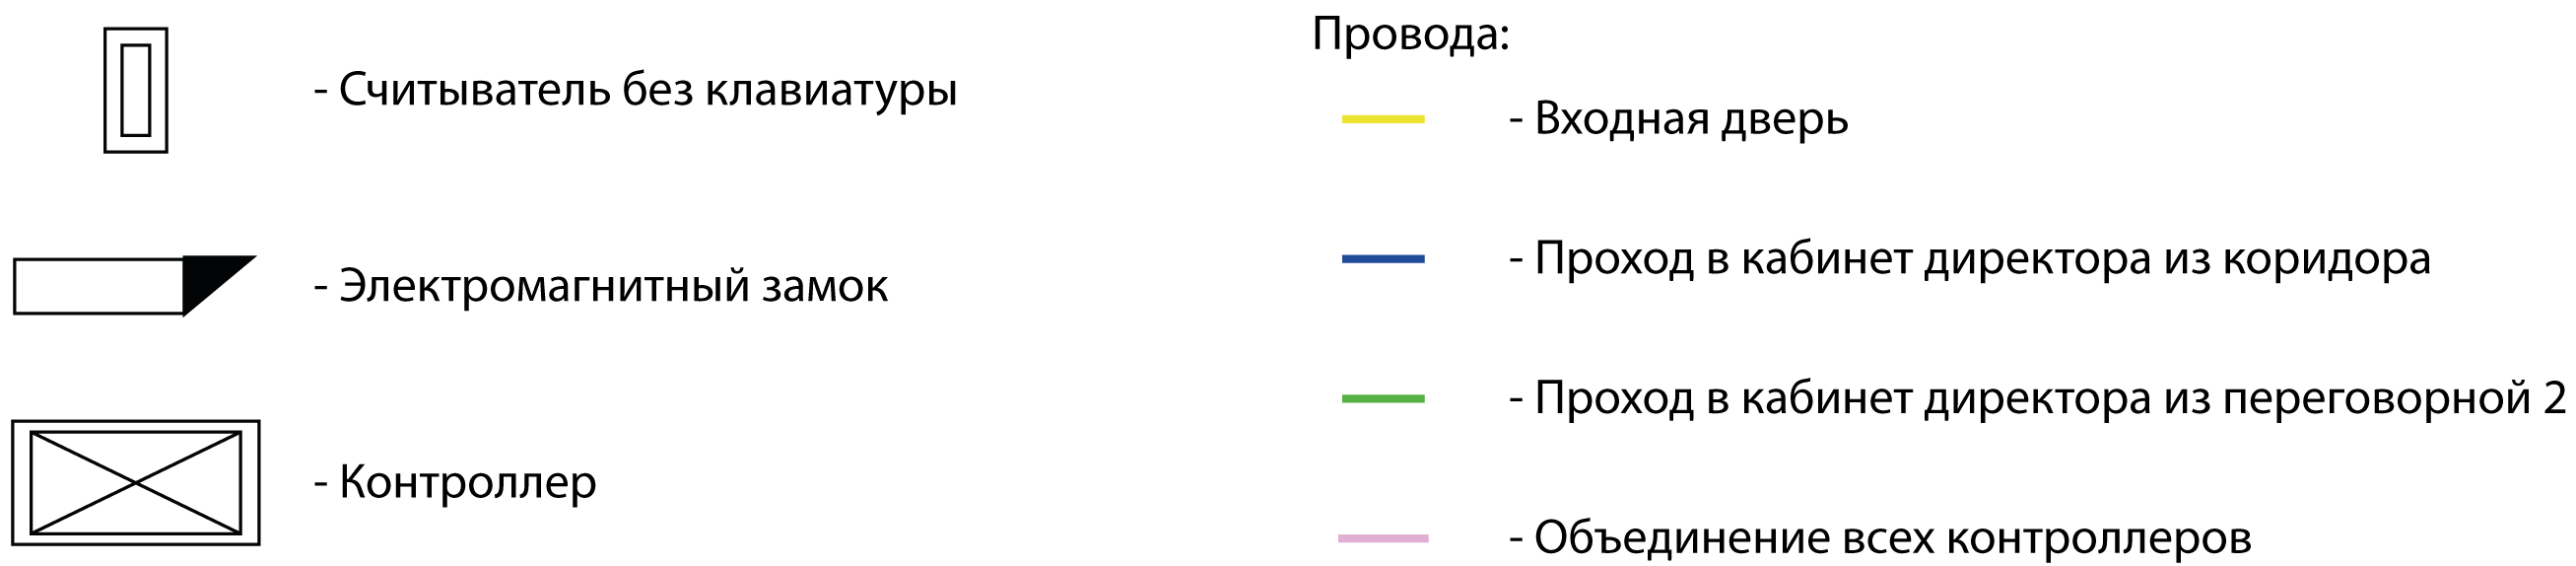
\includegraphics[scale=0.65]{pics/SCUD(mark).png}
    \end{center}
    \textbf{Пояснительная записка}
    \begin{spacing}{1.25}
        В офисе установлено 4 системы контроля и управления доступом:
        \vspace{-1ex}
        \begin{spacing}{0.5}
            \begin{itemize}
                \item на входной двери в офис;
                \item на двери пункта охраны.
                \item на двери в кабинет директора из коридора;
                \item на двери в кабинет директора из переговорной №2.
            \end{itemize}
        \end{spacing}
        Первая система позволяет контролировать приход и уход сотрудников в офис, а также фиксировать время их прибытия. 
        
        Вторая и третья системы охраняют кабинет директора от проникновения, так как это помещение содержит много ценной информации. Каждая из дверей обеспечена отдельным контроллером для того, чтобы в случае проникновения была возможность установить, с какой стороны пришел злоумышленник. 
        
        Четвертая система нужна для того, чтобы в комнату охраны имел доступ только сотрудник охраны и допущенный персонал (например, системный администратор), а также для предотвращения краж сервера системы видеонаблюдения и пульта охранной сигнализации.

        Каждая система состоит из контроллера, электромагнитного замка и 2 считывателей
        без клавиатуры. Использование считывателя без клавиатуры с двух сторон двери обусловлено тем, что сотрудники офисного помещения используют смарт-карты. Это усиливает меры безопасности офисного пространства. Например: если злоумышленник проникнет в офисное помещение, ему будет сложнее выйти через входную дверь, в случае, когда путь через окна будет перекрыт.

        Все системы объединены в единую сеть с целью обмена информацией о перемещениях сотрудников офисного помещения. Данная информация может быть использована для настройки правил доступа к тем или иным помещениям. 
    \end{spacing}

    \vspace{3ex}
    \textbf{Вывод}

    В ходе данной лабораторной работы мы перенесли чертеж офисного помещение с бумажного носителя на электроныый, применив приложение AutoCAD. 

    Мы спроекировали систему охраны, видеонаблюдения, контроля и управления доступом. 

    С помощью программы Illustator данные системы были перенесены на 3 отдельных чертежа помещения.


 
    


    
    


\end{document}